
\chapter{How to Find an Antiderivative }

The Fundamental Theorem of Calculus says that an integral (defined as the area under a curve) can be easily evaluated \integ{via antiderivative}.  However, it turns out to be very difficult and sometimes impossible to find an antiderivative!  In this chapter, we give several commonly used methods for antidifferentiation.

\begin{exercise}{What is an Antiderivative Again? \Coffeecup }
\begin{itemize}
\item Complete the \antider{definition} of antiderivative.  That is, if $f(x)$ is a function, then we say $F(x)$ is an antiderivative of $f(x)$ if and only if... 
\solushun{$$F'(x)=f(x)$$}{.2in}

\item How do you use antiderivatives \antider{to evaluate definite integrals}?  Describe in a short sentence below. 

\vspace*{.2in}

\item Once you found an antiderivative, what could you do to check that it is correct? (Besides just computing it again!)
\AnswerKeyEntry{Saying that $F$ is an antiderivative of $f$ is equivalent to saying the derivative of $F$ is $f$.  That is, $F'(x)=f(x)$.  The Fundamental Theorem of Calculus states that after antidifferentiating the integrand, one can plug the bounds into the antiderivative and take their difference in order to calculate the integral.  Because $F'(x)=f(x)$ by the definition of an antiderivative, a good way to check that your antiderivative $F$ is correct is to take its derivative $F'$. You should get the original function, $f$.}
\end{itemize}
\end{exercise}

\section{The Method of \integ{$u$-Substitution}}
\subsection{Undoing the Chain Rule}\label{undo}
The technique of \antider{$u$-substitution} (affectionately known as ``$u$-sub" from here on) can be seen as the reverse of the chain rule for antiderivatives.

\begin{exercise}{What Was the Chain Rule Again? \Coffeecup }
\begin{itemize}
\item First, write down the chain rule. $$\left(f\left(g(x)\right)\right)'= \hspace{2in} $$ 
\solushun{$$\left(f\left(g(x)\right)\right)'= f'(g(x)) \cdot g'(x)$$}{.1in}

\item Take the antiderivative of both sides of that equation.  $$\int \hspace{1in} \dif x= f\left(g(x)\right)+C \hspace{1in} $$
\solushun{$$\int f'(g(x)) \cdot g'(x) \dif x = \int \left(f\left(g(x)\right)\right)' \dif x= f\left(g(x)\right)+C \hspace{1in} $$}{.1in}
\AnswerKeyEntry{$ \intop f'(g(x)) \cdot g'(x) \dif x = \intop \left(f\left(g(x)\right)\right)' \dif x= f\left(g(x)\right)+C$}
\end{itemize}
\end{exercise}
%
In practice, we often make the substitution $u=g(x)$ to condense the notation.  This will take a nastier integral with respect to $x$ and replace it by a hopefully friendlier integral with respect to $u$.  This process of transforming from $x$ to $u$ involves the following three steps: 
%
\begin{enumerate}
\item {\bf Choose $u$:} Pick $u$ to be equal to some expression involving $x$. Frequently, it is helpful to pick $u$ to be some ``inner function'' in a composition of functions that appears in the integrand.  However, there is a \emph{lot} of freedom regarding what substitution you make.  Some choices of $u$ will be helpful, and others will not be!  It is important to be brave and just try some.
\item {\bf Differentiate $u$:} Once you have a formula for $u$, differentiate with respect to $x$ to get a formula for $\frac{\dif u}{\dif x}$.  This will tell us what the conversion factor is between $x$ units and $u$ units.
\item {\bf Solve for $\dif x$:} Use your derivative to solve for $\dif x$.  Substitute that expression for the $\dif x$ in the integral to replace it with $\dif u$.
\end{enumerate}

For the sake of having this process in a nice little formula box, here is the above paragraph rewritten concisely and precisely.
\FormulaBox{$u$-Substitution}{\begin{tabular}{c}
		$\int f'\left(g(x)\right)\dif x=\int f'(u) \dif u=f(u)+C=f\left(g(x)\right)+C$
	\end{tabular}}

\begin{example}{An Example of Integration via $u$-sub}\label{sup} To evaluate $ \int x \cos\left( x^2\right) \dif x$, we identify $u=x^2$ as a plausible choice based on our recollection of chain rule.  This gives the following change of variables:
\FormulaBox{Three Steps of $u$-Substitution}{\begin{tabular}{c|c|c}
		Choice of $u$ & Differentiate $u$ & Solve for $\dif x$ \\ \hline
		
		$u=x^2$ & $ \frac{\dif u}{\dif x}=2x$ & $\dif x=\frac{1}{2x}\dif u$
	\end{tabular}}

We now replace $x^2$ by $u$ and replace $\dif x$ by $\frac{1}{2x}\dif u$ in our integral.
$$ \int x \cos\left( x^2\right) \dif x = \int x\cdot \cos(u) \frac{1}{2x}\dif u =\frac{1}{2}\int \cos(u) \dif u=\frac{1}{2}\sin(u)+C=\frac{1}{2}\sin\left(x^2\right)+C$$

\end{example}

\begin{exercise}{Checking Our Work \Coffeecup }
As a follow up to the previous example, differentiate the answer to verify that you end up with the original integrand!

$$\frac{\dif}{\dif x}\left(\frac{1}{2}\sin\left(x^2\right)+C\right)=\hspace{4in}$$
\solushun{$$\frac{\dif}{\dif x}\left(\frac{1}{2}\sin\left(x^2\right)+C\right)=\frac{1}{2}\cdot\frac{\dif}{\dif x}\sin\left(x^2\right)+\frac{\dif}{\dif x}C=\frac{1}{2}\cos\left(x^2\right)\cdot 2x+0=x\cos\left(x^2\right) $$}{.1in}

\end{exercise}

\begin{example}{A Trickier $u$-sub}  Suppose we wish to evaluate the following integral:  $$ \int \frac{\sqrt[3]{x}}{\sqrt[3]{x}+1}\dif x$$ One possible approach is to let $u$ be the denominator.  The denominator can be thought of as the ``inner function'' inside a reciprocal function and thus often makes a good choice for $u$.
\FormulaBox{Three Steps of $u$-Substitution}{\begin{tabular}{c|c|c}
		Choice of $u$ & Differentiate $u$ & Solve for $\dif x$ \\ \hline
		
		$u=\sqrt[3]{x}+1$ & $ \frac{\dif u}{\dif x}=\frac{1}{3}x^{-2/3}$ & $\dif x=3x^{2/3}\dif u$
	\end{tabular}}

We now perform the substitutions on the denominator and the $\dif x$.

$$ \int \frac{\sqrt[3]{x}}{\sqrt[3]{x}+1}\dif x= \int \frac{\sqrt[3]{x}}{u}3x^{2/3}\dif u = 3 \int \frac{x}{u}\dif u  $$

At the moment, it seems like things are going very poorly!  We hoped that $x$ in the numerator would nicely cancel out, like it did back in the more civilized age of Exercise \ref{undo}.\ref{sup}.  To fix this, we solve for $x$ in the equation $u=\sqrt[3]{x}+1$ to obtain $x=\left(u-1\right)^3$.  We now substitute that expression for $x$ in the integral.

\begin{align*}
3 \int \frac{x}{u}\dif u & = 3 \int \frac{\left(u-1\right)^3}{u}\dif u \\
& = 3 \int \frac{u^3-3u^2+3u-1}{u}\dif u \\
& = 3 \int u^2-3u+3-\frac{1}{u} \dif u \\
& = u^3-\frac{9}{2}u^2+9u-3\ln|u| + C \\
& = \left(\sqrt[3]{x}+1\right)^3-\frac{9}{2}\left(\sqrt[3]{x}+1\right)^2+9\left(\sqrt[3]{x}+1\right)-3\ln\left|\sqrt[3]{x}+1\right| + C \\
& = x-\frac{3}{2}\sqrt[3]{x}^2+3\sqrt[3]{x}-3\ln\left|\sqrt[3]{x}+1\right| + C \\
\end{align*}

\end{example}

\begin{exercise}{Missing Constants \Coffeecup }
In the above example, all of the constant terms disappeared on the final step!  Was that ok?  
\vspace{.2in}
\end{exercise}

\begin{exercise}{Practice with $u$-sub \Coffeecup \Coffeecup}
\begin{itemize}
\item Evaluate $\int \frac{6x+3}{x^2+x+8} \dif x$.
\solushun{$$\int \frac{6x+3}{x^2+x+8} \dif x = 3\int \frac{2x+1}{x^2+x+8} \dif x $$
$$\text{Let } u=x^2+x+8 $$
$$\text{Then } \dif u = 2x+1 \dif x $$
$$3\int \frac{\dif u}{u} = 3 \ln u + C = 3 \ln \left(x^2+x+8\right)+C $$}{1.5in}
\item Evaluate $\int \frac{\left(\ln(x)\right)^2}{x} \dif x$.
\solushun{$$\text{Let } u=\ln(x) $$
$$\text{Then } \dif u = \frac{1}{x} \dif x $$
$$\int u^2 \dif u = \frac{u^3}{3}+C= \frac{1}{3}\left(\ln (x)\right)^3+C$$}{1.5in}
\item Evaluate $\int x e^{-x^2} \dif x$.
\solushun{$$\text{Let } u=-x^2 $$
$$\text{Then } \dif u = -2x \dif x \text{ and } \dif x = -\frac{1}{2x}\dif u$$
$$\int x e^{-x^2}\left( -\frac{1}{2x}\dif u\right) = -\frac{1}{2}\int e^u \dif u $$
$$-\frac{1}{2}e^u + C = -\frac{1}{2}e^{-x^2} + C$$}{1.5in}
\item Consider the integral  $$\int  e^{\left(x^2\right)} \dif x$$ Explain in words why the substitution $u=x^2$ will not work in this case.  Where do you get stuck? \solushun{$$\text{Let } u=x^2 $$
$$\text{Then } \dif u = 2x \dif x \text{ and } \dif x = \frac{1}{2x}\dif u$$
$$\int  e^{x^2}\left( \frac{1}{2x}\dif u\right) = \frac{1}{2}\int \frac{e^u}{x} \dif u $$
Here we are stuck because there is no way to cancel $x$ and we can't integrate with two variables.\\}{1.5in}
\AnswerKeyEntry{Use the substitutions $u=x^2+x+8, \ln(x),$ and $-x^2$.  In the last case, the $\dif u$ term has nothing to cancel the $x$ with!}
\end{itemize}
\end{exercise}

\begin{exercise}{Create an Integral! \Coffeecup \Coffeecup \Coffeecup}
 Come up with your own integral that can be evaluated by $u$-sub.  Find a partner and trade!  See if you can evaluate each other's integrals with $u$-sub, or explain to your partner why theirs cannot be evaluated using $u$-sub.

\vspace{2in}
\end{exercise}

\subsection{Change of Coordinates and $u$-Substitution}

The method of $u$-substitution is actually a special case of a more general notion, \emph{change of coordinates}.  This will be studied more thoroughly and in more generality in Calculus 3.  

\begin{example}{How $u$-sub Affects Area}

Suppose we wish to compute the following integral: $$\int_{x=0}^{x=4}\sqrt{2x+1} \dif x $$ 
We interpret this as the \integ{area under the curve} $f(x)=\sqrt{2x+1}$ from $x=0$ to $x=4$ as drawn below.  We apply the substitution $u=2x+1$.
This transforms a region in the $xy$-plane to a region in the $uy$-plane.
\begin{center}
\begin{tabular}{c c}
    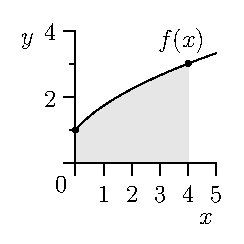
\includegraphics[height=100pt]{ChapterAntidiff/Figures/usubint1.eps}
    %\caption{Graph of $f(x)=\sqrt{2x+1}$} 
	&
    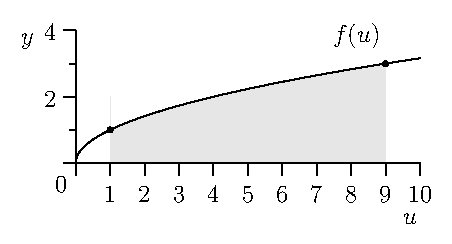
\includegraphics[height=100pt]{ChapterAntidiff/Figures/usubint2.eps}
\end{tabular}
\end{center}

Notice the heights are exactly the same, but the widths have changed by a factor of 2.  Thus to equate the $x$ integral to the $u$ integral, we need to divide the $u$ integral by 2 in order to fix the fact that we doubled all the widths!  In particular, $$\int_{x=0}^{x=4}\sqrt{2x+1} \dif x =\frac{1}{2}\int_{u=1}^{u=9}\sqrt{u} \dif u.  $$
Note that this geometric interpretation corresponds perfectly to what happens in the \integ{Riemann sum} definition of an integral.  For a fixed number of rectangles, the $\Delta x$ in a Riemann sum of the area under $\sqrt{2x+1}$ would be exactly half of the $ \Delta u$ in a corresponding Riemann sum of the area under $\sqrt{u}$.

\end{example}

\begin{exercise}{Relationship between $\Delta x$ and $\Delta u$ \Coffeecup }

\begin{wrapfigure}{r}{0.2\textwidth}
  \centering
  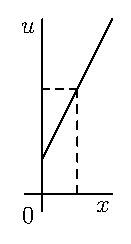
\includegraphics[height=100pt]{ChapterAntidiff/Figures/utox.eps}
  \caption*{Graph of $u=2x+1$, constant derivative 2.}
\end{wrapfigure}
To illustrate the final claim of the example, draw an evenly-spaced four-rectangle Riemann Sum in each of the two shaded regions above.

\begin{itemize}
\item What is your value of $\Delta x$?
\solushun{$$\Delta x = 1$$}{.25in}

\item What is your value of $\Delta u$?
\solushun{$$\Delta u = 2$$}{.25in}

\item Explain where the $u$ bounds of 1 and 9 come from.
\solushun{Since $u=2x+1$, when $x=0$, $u=1$, and when $x=4$, $u=9$. The "$+1$" shifts $u$ 1 unit to the right, just as it would in a graph transformation.\\}{.25in}

\item In the conversion $u=2x+1$, the multiplication by 2 had all the effects described above.  But, why did the ``plus one'' not affect area?  ({\bf Hint:} What would the $u$ bounds have been, and what would the region have looked like, if the ``plus one'' was not there?)
\solushun{Sliding the graph has no effect on its area. If the substitution had been $u=2x$, then the $u$ bounds would have been $0-8$, but the graph would also have started at -1, so the shaded region would be the same in relation to the curve.\\}{.2in}

\item In the figure at right, what aspect of that graph corresponds to the scaling factor between $x$ and $u$?
\solushun{The scaling factor is represented by the slope $\frac{\dif u}{\dif x}$ of the line in the graph at right.\\}{.2in}

\AnswerKeyEntry{To have four intervals in the Riemann sum, $\Delta x$ would be 1 while $\Delta u$ would be 2.  Thus, the width of each rectangle is getting doubled, since to convert between $u$ and $x$ we use the formula $u=2x+1$.  The ``plus one'' merely slides all the rectangles one unit to the right, but it does not stretch their width at all, so it does not affect their area.  Thus, the slope of the graph of $u=2x+1$ is the only thing that mattered regarding our conversion between $x$ and $u$.  That is to say, the quantity $\dif u/ \dif x$ gives us the scaling factor.}
\end{itemize}
\end{exercise}

 The moral to the story is that the scaling factor between $\Delta x$ and $\Delta u$ is in fact the derivative of $u$ with respect to $x$.   In order to translate from $x$ to $u$ in our integral, we must divide by $\frac{du}{dx}$. In this case, that was just the constant 2. 
What is fascinating is that this approach of dividing off by the scaling factor still works, even when the scaling factor is not just a constant.  Hence if we use $u=x^2$, we must divide by $\frac{\dif u }{\dif x}=2x$, as we do in many of the above examples.  It is still a scaling factor, but one that changes depending on the input!  

\begin{exercise}{Looking Graphically at a $u$-sub \Coffeecup \Coffeecup}

% \begin{wrapfigure}{r}{0.2\textwidth}
% 	\centering
%  	%
\begin{asy}
	size(100);  
    import graph;
    
    real f(real x)
    {
        return x^2;
    }
           
    xlimits(0, 3);
	ylimits(0, 4);
    draw(graph(f,0,2,n=400), linewidth(.75bp), arrow=Arrow(HookHead));
    
    draw((0,0)--(1/4,0), linewidth(.5bp), arrow=Arrow(HookHead));
    draw((1/4,1/16)--(1/2,3/16), linewidth(.5bp), arrow=Arrow(HookHead));
    draw((1/2,1/4)--(3/4,1/2), linewidth(.5bp), arrow=Arrow(HookHead));
    draw((3/4,9/16)--(1,15/16), linewidth(.5bp), arrow=Arrow(HookHead));
    draw((1,1)--(5/4,3/2), linewidth(.5bp), arrow=Arrow(HookHead));
    draw((5/4,25/16)--(3/2,35/16), linewidth(.5bp), arrow=Arrow(HookHead));
    draw((3/2,9/4)--(7/4,3), linewidth(.5bp), arrow=Arrow(HookHead));
    
	yaxis("$u$", -.5, 4);
	xaxis("$x$", -.5, 2);
    labelx("$0$",0,1S+1W);
    
\end{asy}
%     \includegraphics[height=100pt]{ChapterAntidiff/utoxsquared.eps}
%  	\caption*{Graph of $u=x^2$, changing derivative of $2x$.}
% \end{wrapfigure}
We now look at a case where the scaling factor depends on $x$.
\begin{itemize}
\item Plot a graph of the function $f(x)=x\sin(x^2)$ on the domain $[0,3]$. (You may use a graphing utility to assist you.)
\solushun{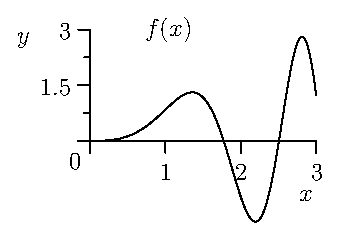
\includegraphics[height=100pt]{ChapterAntidiff/Figures/solxsinx_cropped.eps}\\}{.7in}
\end{itemize}
\begin{minipage}[l]{.75\textwidth}
\begin{itemize}
\item  Plot a graph of the function $h(u)=\sqrt{u}\sin(u)$ on the domain $[0,9]$. (You may use a graphing utility to assist you.)
\solushun{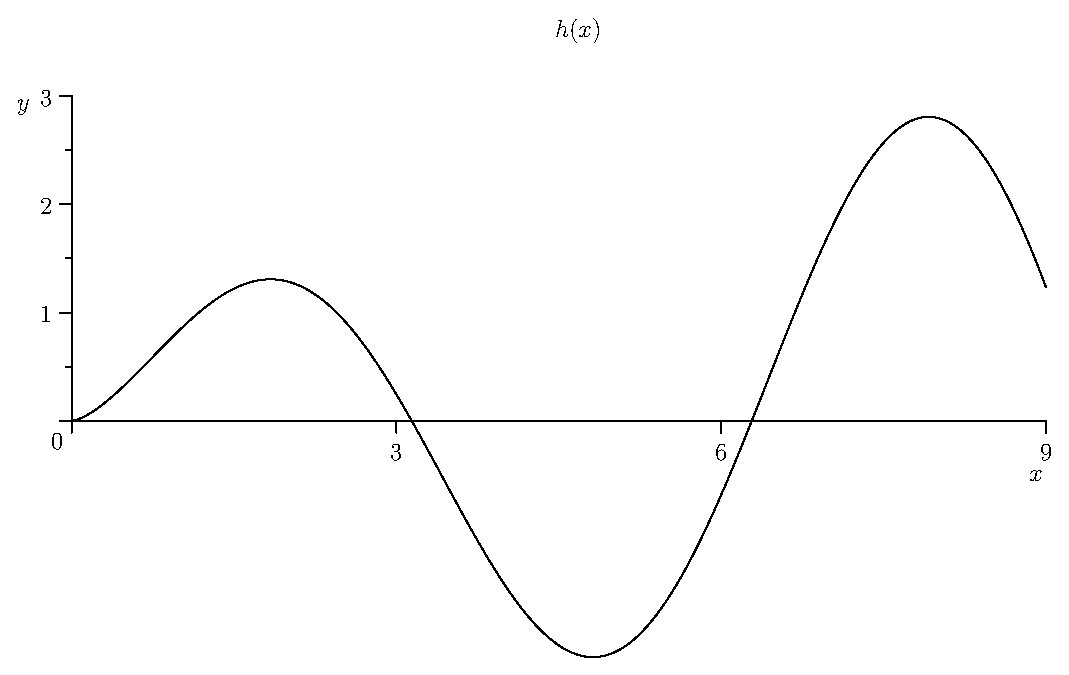
\includegraphics[height=100pt]{ChapterAntidiff/Figures/solusinu_cropped.eps}\\}{.5in}

\item Can you see the horizontal scaling factor change at different points of the graph?  How stretched out does it seem to be at $x=1$?  How stretched out does it seem to be at $x=3$?
\solushun{At $x=1$, the scaling factor is about 1. At $x=3$ the scaling factor is about 9.\\}{.5in}

\item Show algebraically that $u=x^2$ is the substitution that turns that function $f(x)$ into the corresponding function $h(u)$.
\solushun{$$\text{Let } u=x^2 $$
$$\text{Then } x=\sqrt{u}$$
$$\text{Substituting: } x \sin x^2 = \sqrt{u} \sin u$$}{.5in}

\item Evaluate the integral $\int_{x=0}^{x=3}x\sin(x^2)\dif x$.
\solushun{$$\text{Let } u=x^2 \text{, then } \frac{\dif u}{ \dif x} = 2x \text{, and } \dif x = \frac{\dif u}{2x}$$
$$\text{Substituting into the original function:}$$
$$\int_{x=0}^{x=3}x\sin(u)\frac{\dif u}{2x} = \frac{1}{2}\int_{u=0}^{u=9}\sin(u)\dif u = \frac{1}{2} \left[ -\cos (u)\right]_0^9 = \frac{1}{2}\left(-\cos9 + 1\right) \approx 0.955$$}{.5in}

\item In the figure at right, what aspect of that graph corresponds to the scaling factor between $x$ and $u$? 
\solushun{The slope at each point, $\frac{\dif u}{\dif x} = 2x $, is the scaling factor.}{.5in}

\end{itemize} 
\end{minipage}
 \begin{minipage}[r]{0.2\textwidth}
 	\centering
  	%\vspace*{1.75in}
     \includegraphics[height=100pt]{ChapterAntidiff/Figures/utoxsquared.eps} \\
     Graph of $u=x^2$, changing derivative of $2x$.
 \end{minipage}
 
 \AnswerKeyEntry{The definite integral evaluates to roughly 0.95.  The horizontal scaling factor at each $x$-coordinate should correspond to the derivative $\dif u /\dif x$ at each point. }
 
\end{exercise}

\subsection{\trigfunctions{Antiderivatives} of the Six Trig Functions}\label{SixTrigAntiderivatives}

In Calculus I, we found the derivatives of all six trig functions.  List those below.

\begin{exercise}{Recalling the Derivatives of the Six Trig Functions \Coffeecup}
Write the derivative of each of the following trig functions:
\begin{itemize}
\item $\frac{\dif}{\dif x}\left(\sin(x) \right)=$
\item $\frac{\dif}{\dif x}\left(\cos(x) \right)=$
\item $\frac{\dif}{\dif x}\left( \tan(x)\right)=$
\item $\frac{\dif}{\dif x}\left( \cot(x)\right)=$
\item $\frac{\dif}{\dif x}\left( \sec(x)\right)=$
\item $\frac{\dif}{\dif x}\left( \csc(x)\right)=$
\end{itemize}
\solushun{\begin{itemize}
\item $\cos(x)$
\item $-\sin(x)$
\item $\sec^2(x)$
\item $-\csc^2(x)$
\item $\sec(x)\tan(x)$
\item $-\csc(x)\cot(x)$
\end{itemize}}{0in}
\end{exercise}

From these, we easily obtain the antiderivatives of sine and cosine.

\begin{exercise}{Integrals of Sine and Cosine \Coffeecup}
Use the derivatives above to compute the following antiderivatives.
\begin{itemize}
\item $\int \sin(x) \dif x =$
\item $\int \cos(x) \dif x =$
\end{itemize}
\solushun{\begin{itemize}
\item $\int \sin(x) \dif x = -\cos(x) + C$
\item $\int \cos(x) \dif x = \sin(x) + C$
\end{itemize}}{0in}
\end{exercise}

For tangent and cotangent, we need $u$-sub.
\begin{example}{Antiderivative of Tangent}
We compute the \tangent{antiderivative} of tangent by rewriting as $\tan(x)=\frac{\sin(x)}{\cos(x)}$ and then using the substitution $u=\cos(x)$.  Differentiating both sides produces $\dif x = \frac{\dif u}{-\sin(x)}$.  We now apply these substitutions:
\begin{align*}
\int \tan(x) \dif x &= \int \frac{\sin(x)}{\cos(x)}\dif x \\ 
&= \int \frac{\sin(x)}{u}\frac{\dif u}{-\sin(x)} \\
&= -\int \frac{1}{u}\dif u \\
&= -\ln|u|+C \\
&= -\ln|\cos(x)|+C
\end{align*}
\end{example}

The method used to antidifferentiate tangent can be adapted to also antidifferntiate cotangent.
\begin{exercise}{Integral of Cotangent \Coffeecup \Coffeecup}
Find the antiderivative of cotangent.  
$$\int \cot(x) \dif x = \hspace*{3in}$$
\solushun{$$\text{Let } u = \sin(x) \text{, then } \dif x = \frac{\dif u}{\cos x}$$
 \begin{align*}
\int \cot(x) \dif x &= \int \frac{\cos(x)}{\sin(x)}\dif x \\ 
&= \int \frac{\cos(x)}{u}\frac{\dif u}{\cos(x)} \\
&= \int \frac{1}{u}\dif u \\
&= \ln|u|+C \\
&= \ln|\sin(x)|+C
\end{align*}
 }{2in}
\end{exercise}

The \secant{antiderivative} of secant is much trickier!  The process is not intuitive and requires a rabbit out of a hat.
\begin{example}{Integral of Secant} 
Since multiplication by 1 does not change the integrand, we are free to multiply by 1 whenever it is helpful.  Here, it turns out to be helpful to multiply by $\frac{\sec(x)+\tan(x)}{\sec(x)+\tan(x)}$.  This is the rabbit.
\begin{align*}
\int \sec(x)\dif x &=\int \sec(x)\frac{\sec(x)+\tan(x)}{\sec(x)+\tan(x)} \dif x \\
&=\int \frac{\sec^2(x)+\sec(x)\tan(x)}{\sec(x)+\tan(x)} \dif x \\
&=\int \frac{\sec^2(x)+\sec(x)\tan(x)}{u} \frac{1}{\sec(x)\tan(x)+\sec^2(x)}\dif u \\
&=\int \frac{1}{u}\dif u \\
&=\ln|u|+C \\
&=\ln|\sec(x)+\tan(x)|+C
\end{align*}
\end{example}

The above method can be adapted to antidifferentiate cosecant.
\begin{exercise}{Integral of Cosecant \Coffeecup \Coffeecup}
Find the antiderivative of cosecant.  
$$\int \csc(x) \dif x = \hspace*{3in}$$
\solushun{ \begin{align*}
\int \csc(x)\dif x &=\int \csc(x)\frac{\csc(x)+\cot(x)}{\csc(x)+\cot(x)} \dif x \\
&=\int \frac{\csc^2(x)+\csc(x)\cot(x)}{\csc(x)+\cot(x)} \dif x \\
&=\int \frac{\csc^2(x)+\csc(x)\cot(x)}{u} \frac{1}{-\csc(x)\cot(x)-\csc^2(x)}\dif u \\
&=-\int \frac{1}{u}\dif u \\
&=-\ln|u|+C \\
&=-\ln|\csc(x)+\cot(x)|+C
\end{align*}}{2in}
\vspace*{2in}
\end{exercise}
